\chapter{Introduction and Theory Overview} \label{chap:1}

\section{Introduction}
The analysis is aim at searching for heavy resonances decaying to a pair of Higgs
bosons in the four b quark final state using 35.9$fb^{-1}$ proton-proton collison data at center-of-mass energy 13 TeV collected with the CMS detector at the LHC. The figure 1.1 shows the feynman diagram of the channel. 

The Higgs tagging process uses the b-tagging algorithm, N-subjetness variable, and the mass of the jets. The analysis is searching for a bump in the dominant background of multi-jet events.


\begin{figure}[t]
  \begin{center}

    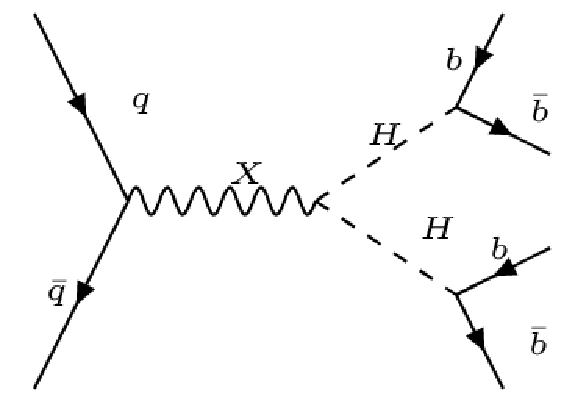
\includegraphics[width=0.5\textwidth]{Figures/Screenshot_20170601_160641.pdf} 
    \end{center}
  \caption{The feynman diagram of q$\bar{q}$ $\rightarrow$ X $\rightarrow$ HH $\rightarrow$ $b\bar{b}b\bar{b}$.}
\end{figure}

In \autoref{chap:1}, an overview of Wrapped Extra Dimension theory, signal model, and motivation is presented. In \autoref{chap:2}, the LHC and the CMS detector are simply introduced. In \autoref{chap:3}, the information of the data and the Monte Carlo Simulation is shown along with the comparison of shape of each discripant variable. The reconstruction and the selection of the event is also fully detailed. In \autoref{chap:4}, the background estimation method based on data driven is presented. All sysyematic uncertainted considered is documented in \autoref{chap:5}. Finally, the result of 95$\% $ CL$_{s}$ upper limit of cross section $\times$ branch ratio is shwon in \autoref{chap:6}. 

\section{Theory}
%http://dx.doi.org/10.1016/j.physletb.2012.08.021
%http://www.sciencedirect.com/science/article/pii/S037026931200857X

The discovery of the boson whose mass around 125 GeV and with properties close to Higgs mechanism in the standard model (SM) has incited the search under Higgs potential including Higgs self-coupling\citep{jetarea_fastjet_pu,HiggsdiscoveryAtlas}. Especially, it is a channel worth exploring and finding new physic beyond the SM. 
Targeting heavy resonance, the model Wrapped Extra Dimension is considered. 

\subsection{Wraped Extra Dimension} 

%https://journals.aps.org/prl/pdf/10.1103/PhysRevLett.83.3370
To solve the hierarchy problem, Wrapped Extra dimension proposed by Randall and Sundrum postulates a scenario that the SM particles and forces associating with gravity force are confined to a four-dimension subspace within (4+n)-dimension spacetime, referred to as "3-brane", 
to explain the fact that we do not see experimental signs of the extra dimensions\citep{Randall:1999ee}.  The spacetime metrix takes the form\citep{Oliveira:2014kla}:

\begin{equation} \label{eq1}
\begin{split}
ds^2 = e^{-2\sigma(\phi)}\eta_{\mu\nu}dx^{\mu}dx^{\nu} + r^2_{c}d\phi^2, 
\end{split}
\end{equation}
where $\mu$ and $\nu$ run over 1, 2, 3, and 4, and $\phi$ is the fifth dimension. Its classical action is 

\begin{equation} \label{eq1}
\begin{split}
S = S_{Gravity}+S_{TeV}+S_{Planck}+S_{Matter},
\end{split}
\end{equation},
where $S_{Gravity}$ is the action of bulk gravity, and $S_{Matter}$ is the action of matter field. The actions can be written as:

\begin{equation} \label{eq1}
\begin{split}
S_{i=TeV/Planck}=-\int d^4x \sqrt{g(\phi =0,\pi)}\Lambda_{i=TeV/Planck}\\
S_{Gravity}=\int d^4 \int ^{\pi}_{\pi} d\phi \sqrt{g}(-\Lambda_{bulk}+2M^3_{5}R),
\end{split}
\end{equation}
where $\Lambda$ is hte vacuum energy density, R is Ricci metrix. We arrive at:

\begin{equation} \label{eq1}
\begin{split}
\sigma(\phi)=r_{c}|\phi | \sqrt{\frac{-\Lambda}{24M^2_5}}\equiv r_c|\phi |k \\
k\equiv  \sqrt{\frac{-\Lambda}{24M^2_5}}, \\
\end{split}
\end{equation}
where k is referred as curvature factor. We can integrate the fifth dimension and get four-dimension Planck mass: 
\begin{equation} \label{eq1}
\begin{split}
\bar{M}^2_{Pl}=\frac{M^3_5}{k}(1=e^{-2\pi kr_c}).
\end{split}
\end{equation}

Finally, we get the spacetime metrix:  
\begin{equation} \label{eq1}
\begin{split}
ds^2 = e^{-2kr_c\phi}\eta_{\mu\nu}dx^{\mu}dx^{\nu} + r^2_{c}d\phi^2, 
\end{split}
\end{equation}


where k is a scale of the order of the Planck scale, xm are
coordinates for the familiar four dimensions, while 0 $\leq$ $\phi$ $\leq$ $\pi$ is the coordinate for an extra dimension, which is
a finite interval whose size is set by $r_c$. The exponential is the source of large hierarchy between weak and the observed Planck scale.  


%https://journals.aps.org/prl/pdf/10.1103/PhysRevLett.83.4922
%https://arxiv.org/pdf/hep-ph/9911406.pdf

%https://arxiv.org/pdf/hep-ph/9909255.pdf
%https://arxiv.org/pdf/hep-ph/0701186.pdf
%https://arxiv.org/pdf/hep-ph/0701150.pdf
There are models predicting the existence of new particles, such as spin-0 radion and spin-2 graviton\citep{Davoudiasl:1999jd,Agashe:2007zd,Fitzpatrick:2007qr}. For example, a radion scalar is added to stablize the $r_c$ in RS theory without a fune-tuning of parameters\citep{Goldberger:1999uk}. Other model proves that
a radion field can remove the constraints between two branes without a stablized radius\citep{Csaki:1999mp}, and that 
%https://arxiv.org/pdf/hep-th/0008151.pdf
a radion scalar can exist with radus stabilization in bulk scalar field while assuming stabilization exists\citep{Csaki:2000zn}.
A possible mixing of the radion which is the only graviscalar in RS model and the Higgs is proposed\citep{Giudice:2000av}.
%https://arxiv.org/pdf/hep-ph/0002178.pdf
However, according to the latest experimental data, the mixing is expected to be small. Therefore, the contribution of the mixing is not considered in this analysis\citep{Desai:2013pga}.
%https://arxiv.org/pdf/1307.3765.pdf

We follow the ref.\citep{Agashe:2013kyb} to calculate the cross section of bulk graviton.
\begin{equation} \label{eq1}
\begin{split}
gg \rightarrow KK graviton \rightarrow ZZ, WW, hh (and t\bar{t}, b\bar{b}) \\
\textit{L}_{prod.} = 0.053 (\frac{k}{M_{Pl}M_{G}})\eta^{\mu\alpha}\eta^{\nu\beta}h^{(1)}_{\alpha\beta}T^{gluon}_{\mu \nu}(x), 
\end{split}
\end{equation}
where the $M_G$ is the mass of KK graviton, and $T^{gluon}_{\mu \nu}$ is four-dimesion four-momentum of SM gluon. The implementation of the calcuation is described in ref.\citep{Oliveira:2014kla}. The model which is capable of calculating the correction of next-to-leading-order QCD induced spin-2 particle is used. The cross section is calculated by \textsf{MG5\_aMC@NLO}.
Because of the Higgs-like property of radion, the cross section of radion is calculated by rescaling the cross section of Higgs like particle\citep{Agashe:2013kyb,AN-16-300}. The production of Higgs-like particle by gluon-gluon fusion is followed by ref.\citep{Catani:2003zt,Heinemeyer:2013tqa}, which is calcuated in next-to-next-to-leading-order QCD induced soft-gluon resummation. The Higgs-like calculation is up to 1 TeV, and it is constant for mass above 1 TeV. The cross section of radion is based on the cross section of Higgs-like multiplied by k factor. 
In the calcuation of both signal, CTEQ6LPDF is used\citep{Nadolsky:2008zw}.  

\subsection{Motivation} 
%https://arxiv.org/pdf/1512.04357.pdf
There are models predicting heavy resonances decaying into VV\citep{Brehmer:2015dan}.
%https://arxiv.org/abs/1506.00962
%https://arxiv.org/abs/1503.04677
%https://arxiv.org/abs/1409.6190
%https://arxiv.org/abs/1405.1994
Several researches on these channels are performed in both CMS and ATLAS.
There are also the combinations of these analyses\citep{Khachatryan:2014hpa,ATLASZV,ATLASWV,ATLASVV}.
%https://arxiv.org/abs/1405.3447
%https://arxiv.org/abs/1512.05099
The combination from ATLAS excludes the resonance of Bulk Graviton from below 810 GeV at $\sqrt{s}$ = 8 TeV\citep{Aad:2015ipg}, and despit the combination from CMS fails to exclude any mass spectum of Bulk Graviton given a less sensitive model, it sets the upper limit of 10 fb of cross section of Bulk Graviton through $M_X$ from 600 to 2500 GeV at $\sqrt{s}$ = 8 TeV\citep{CMSZVWV}.
%https://arxiv.org/pdf/1503.04114.pdf
%https://arxiv.org/pdf/1506.00285.pdf
Searches for Bulk Graviton decaying into HH in four b-flavored quarks final state have been perfromed by CMS and ATLAS at $\sqrt{s}$ = 8 TeV\citep{Khachatryan:2015year,Aad:2015uka}. They exlude the mass region below 830 and 720 GeV respectively. The intermediate region of the mass of heavy resonances ( $M_X \thickapprox$ 2 TeV ) is left interesting to be explored.
 



%
%\begin{figure}[t]
%  \centering
%  \begin{tabular}{cc}
%    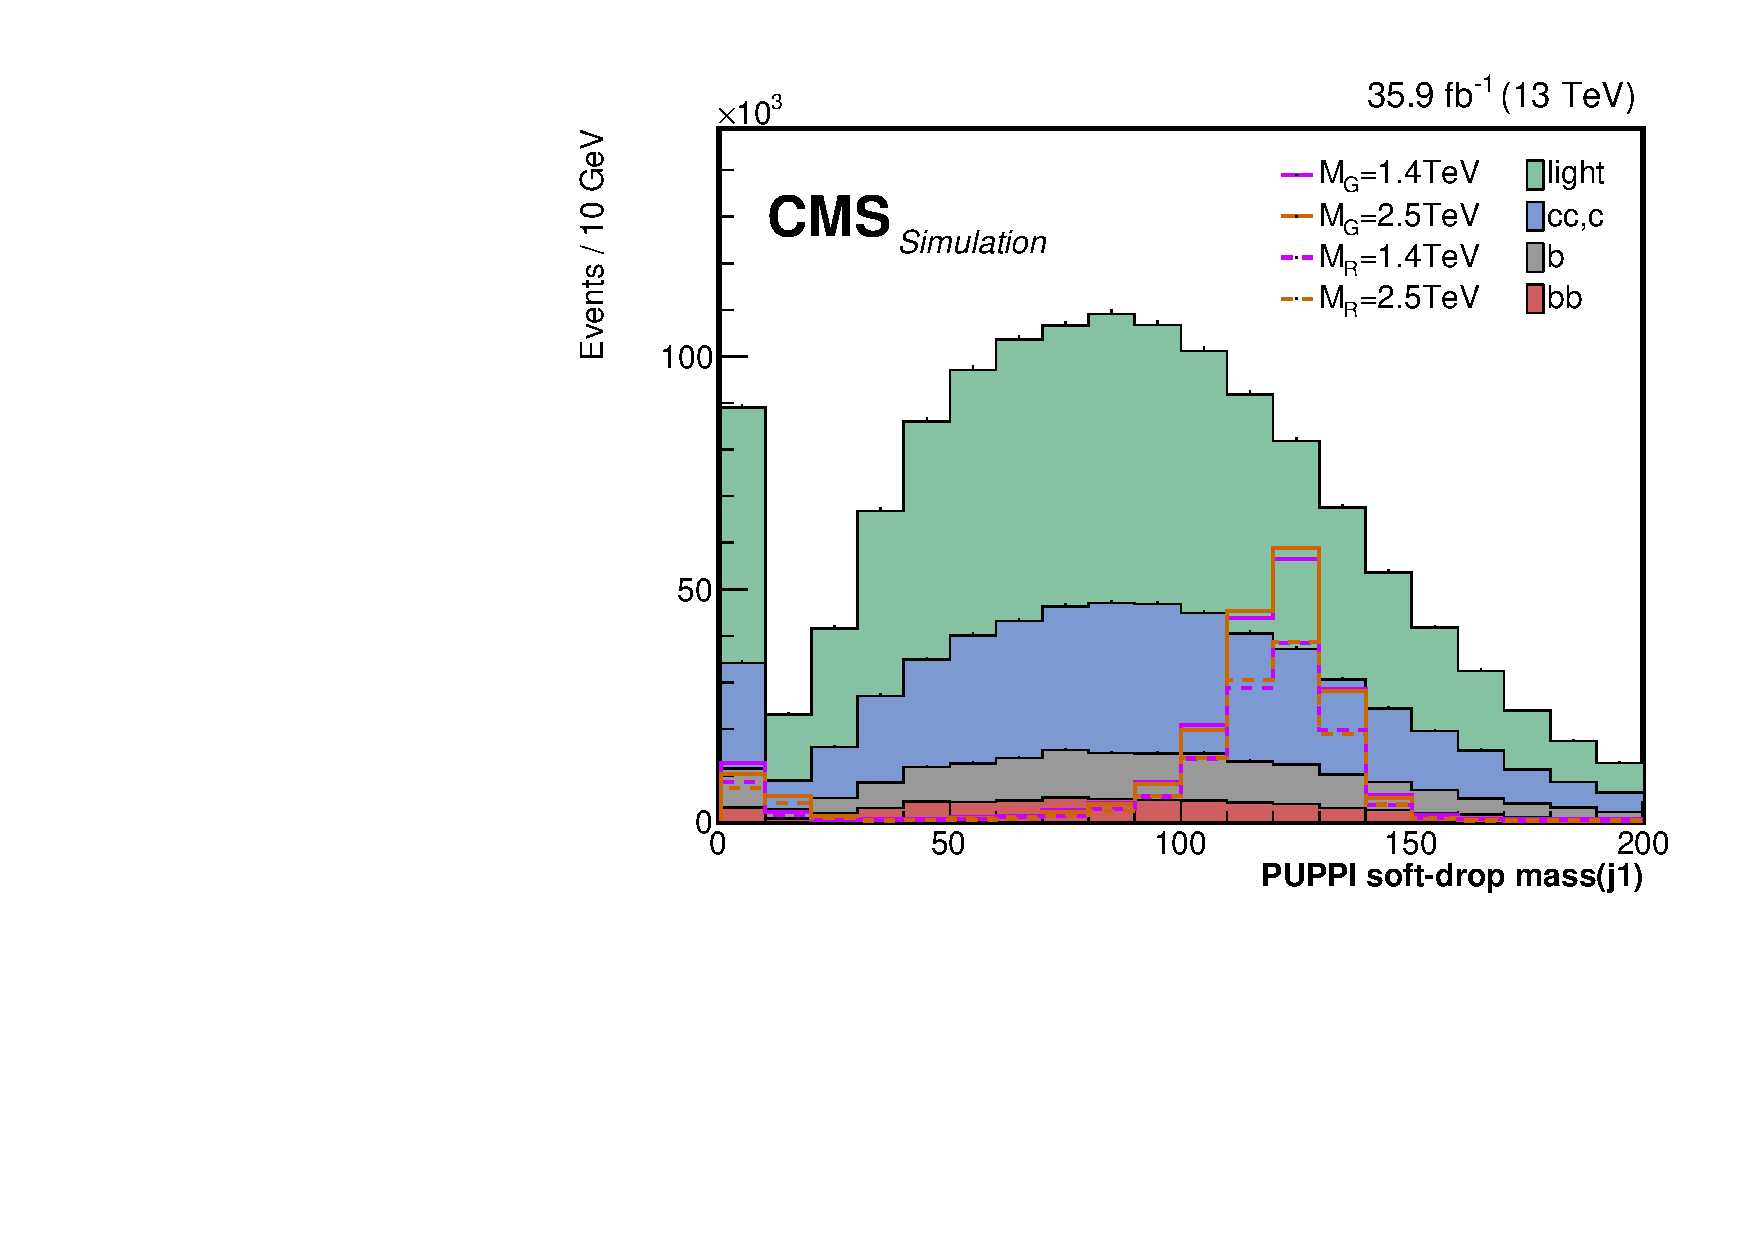
\includegraphics[width=0.5\textwidth]{Figures/MC_N1/puppiSDMassThea_j0.pdf} &
%    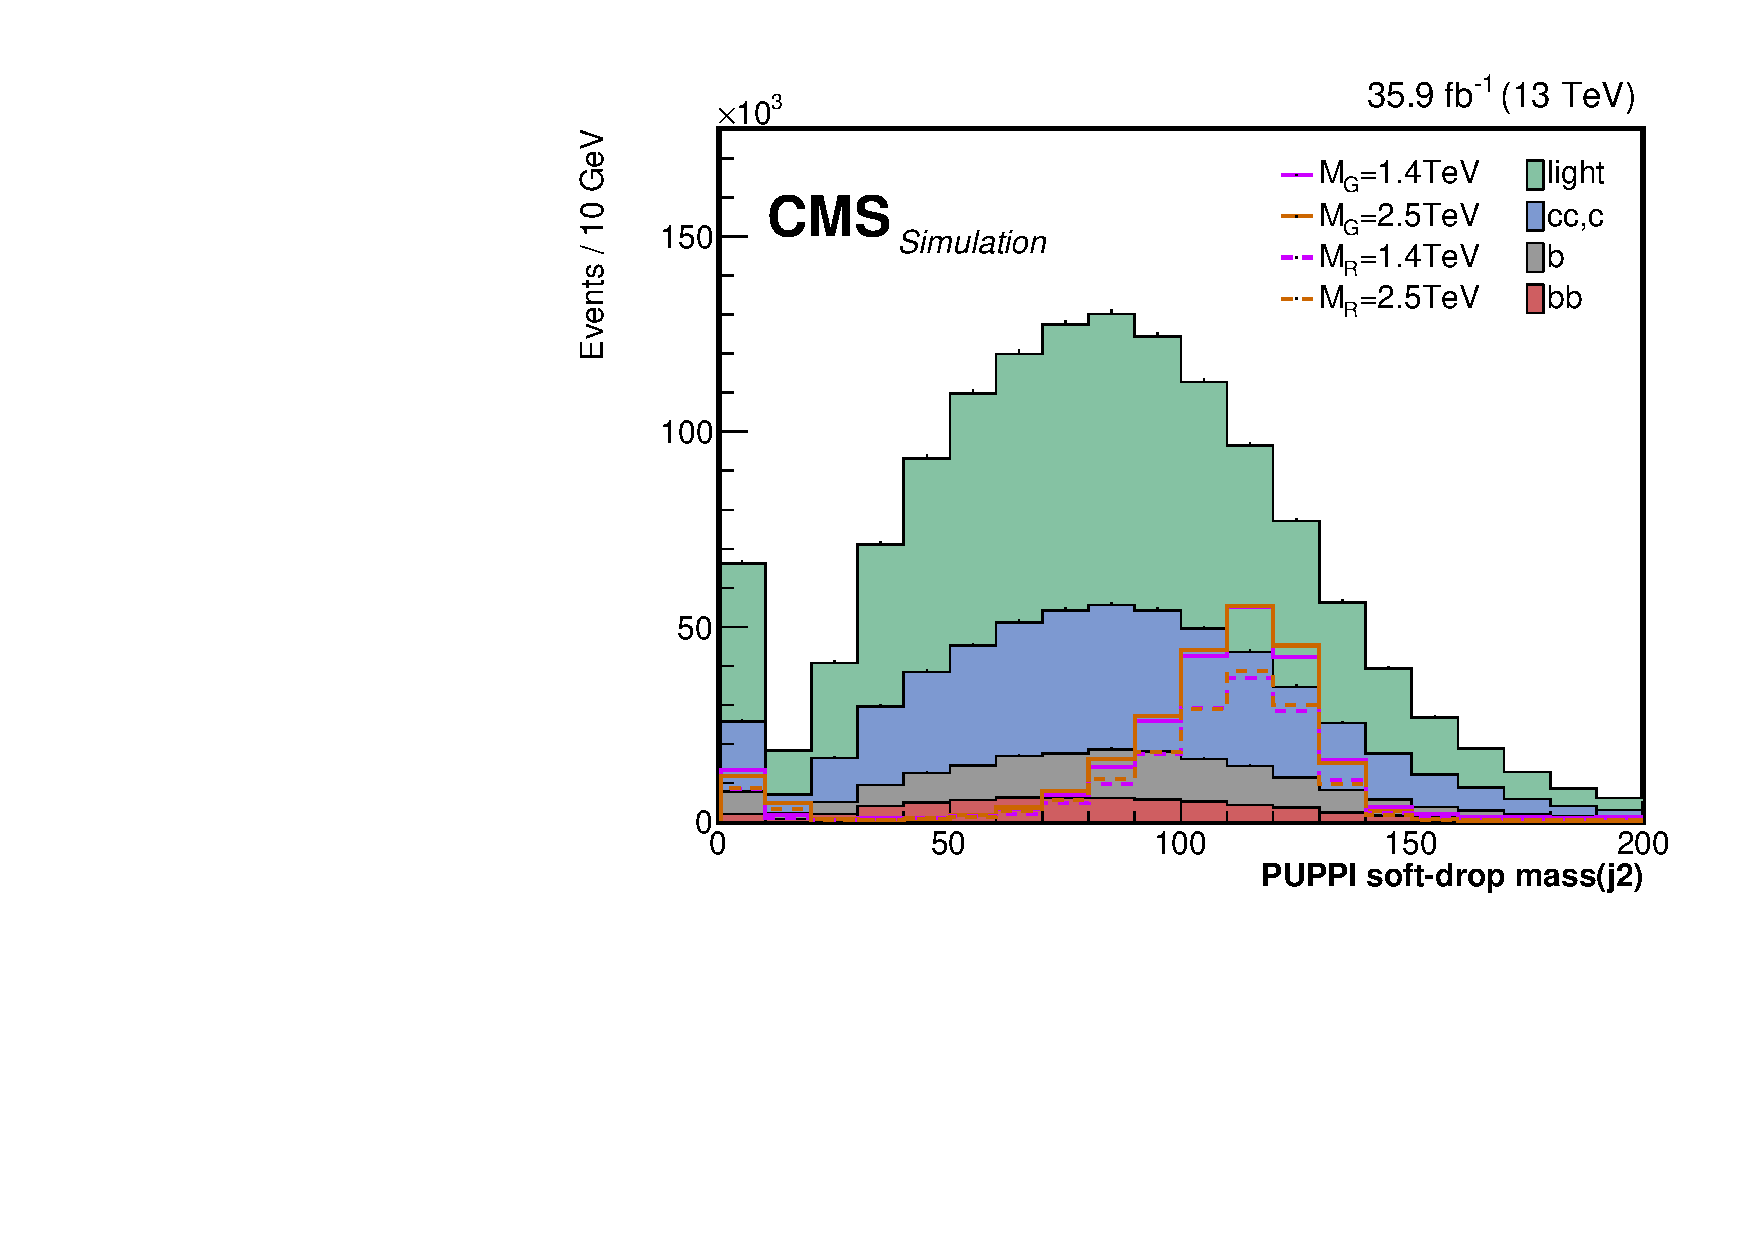
\includegraphics[width=0.5\textwidth]{Figures/MC_N1/puppiSDMassThea_j1.pdf} \\
%     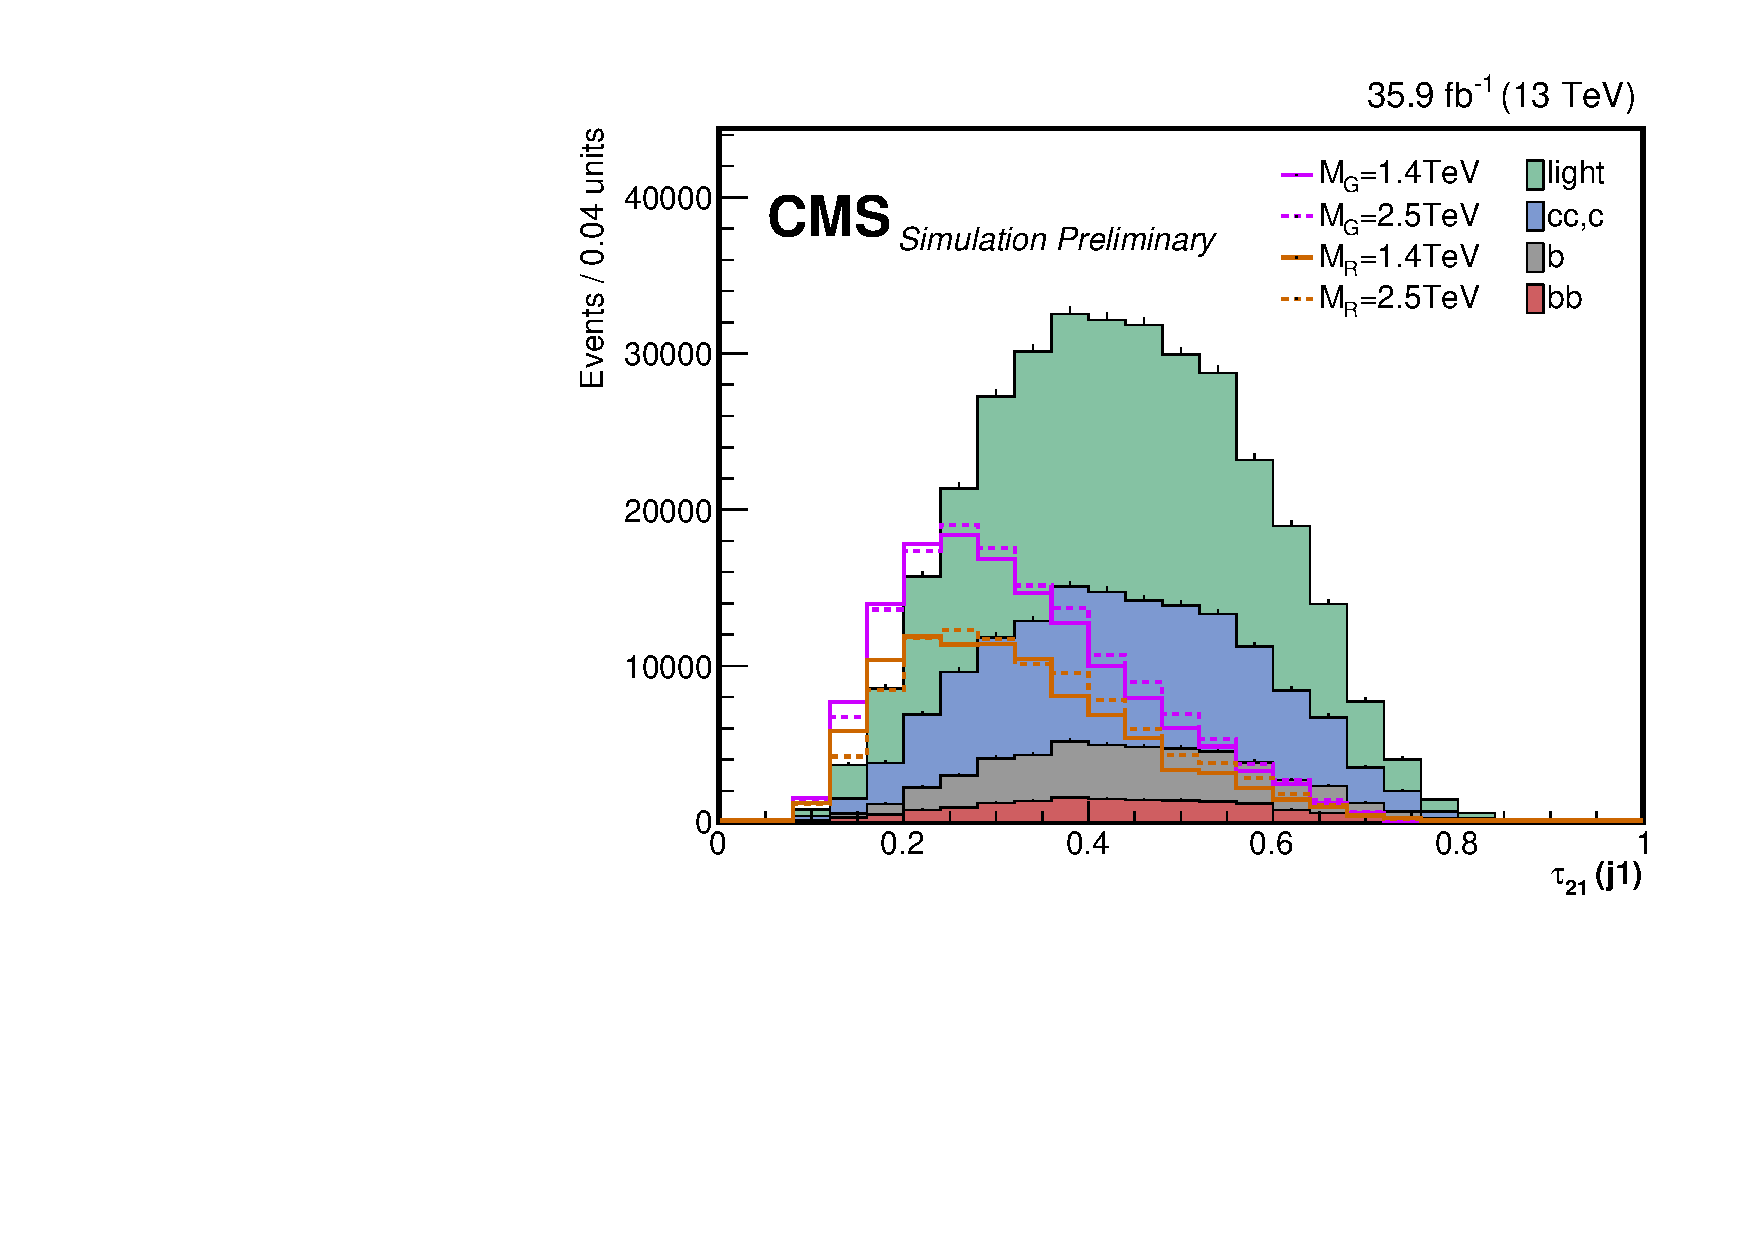
\includegraphics[width=0.5\textwidth]{Figures/MC_N1/puppiTau21_j0.pdf} &
%    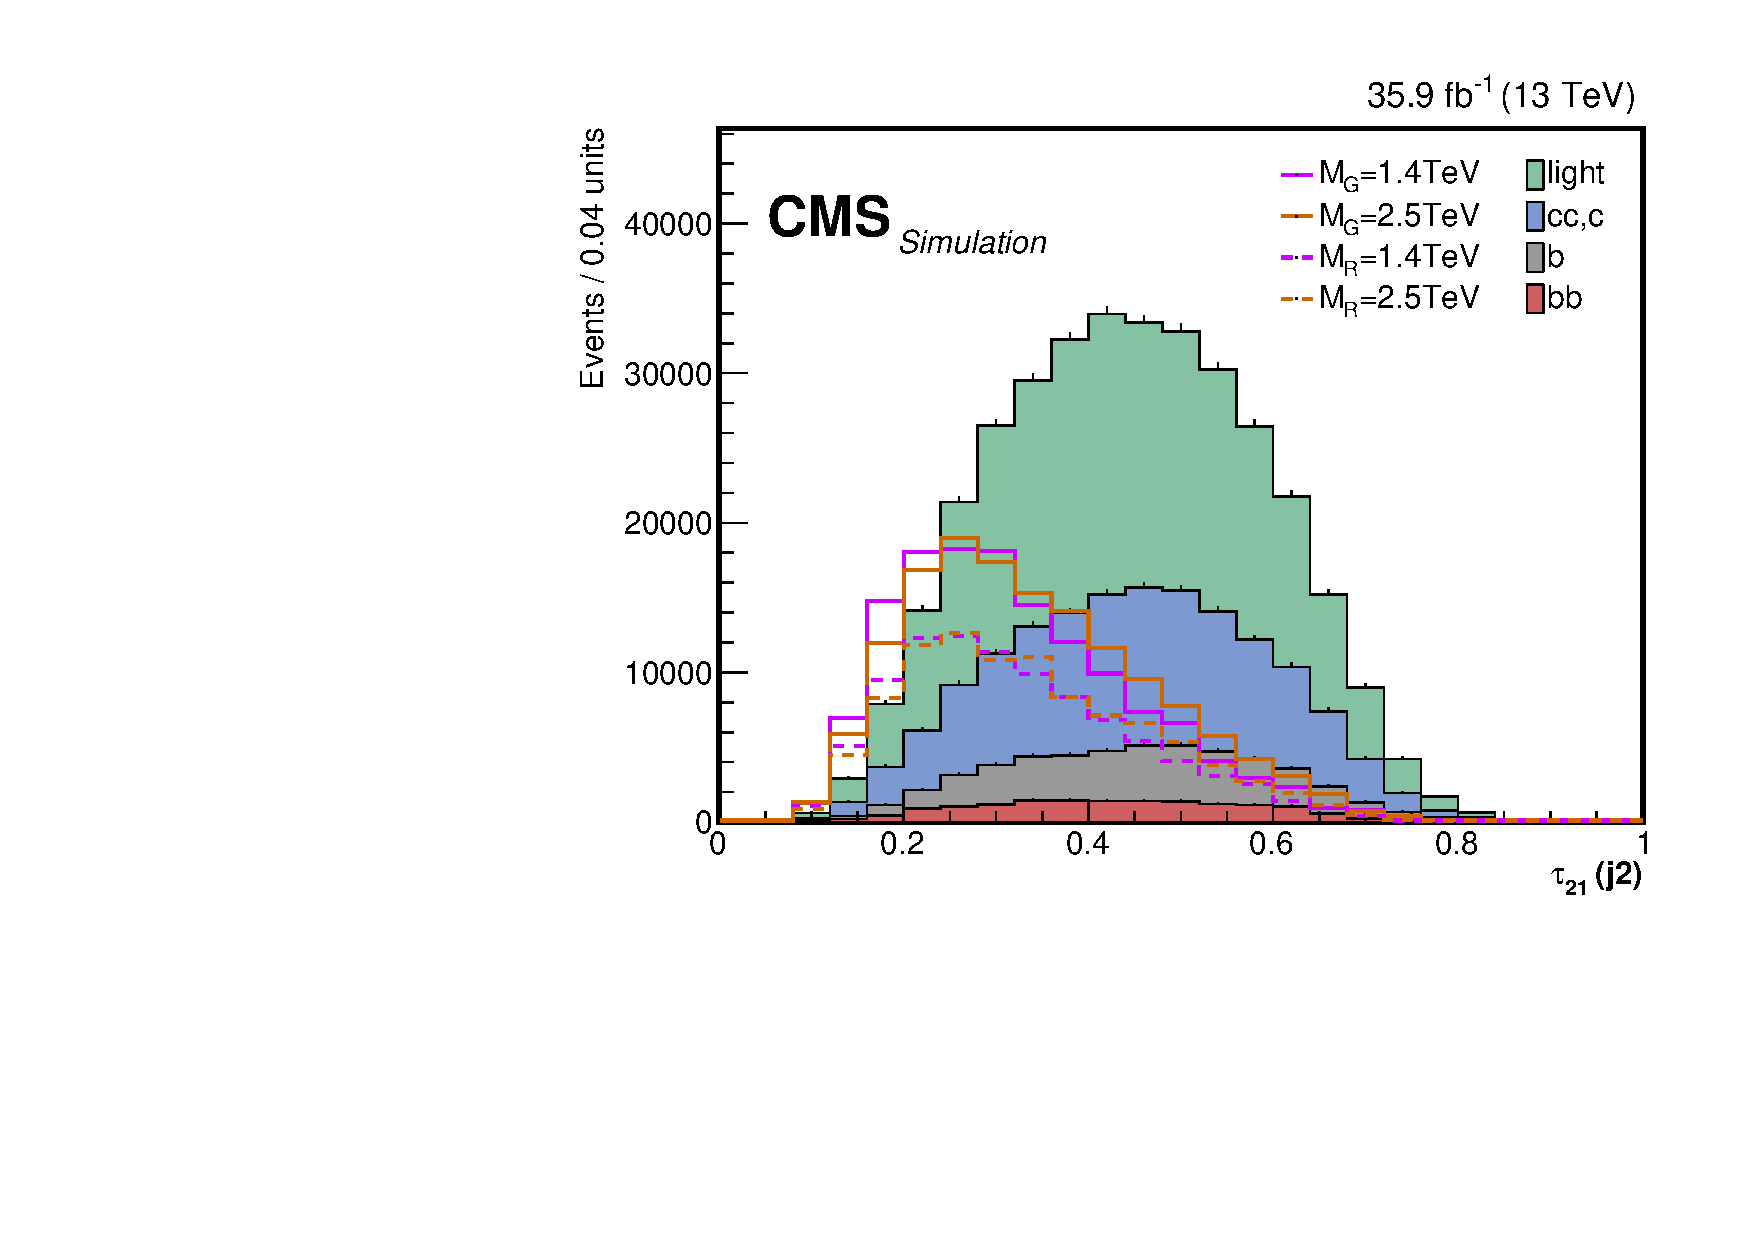
\includegraphics[width=0.5\textwidth]{Figures/MC_N1/puppiTau21_j1.pdf} \\
%     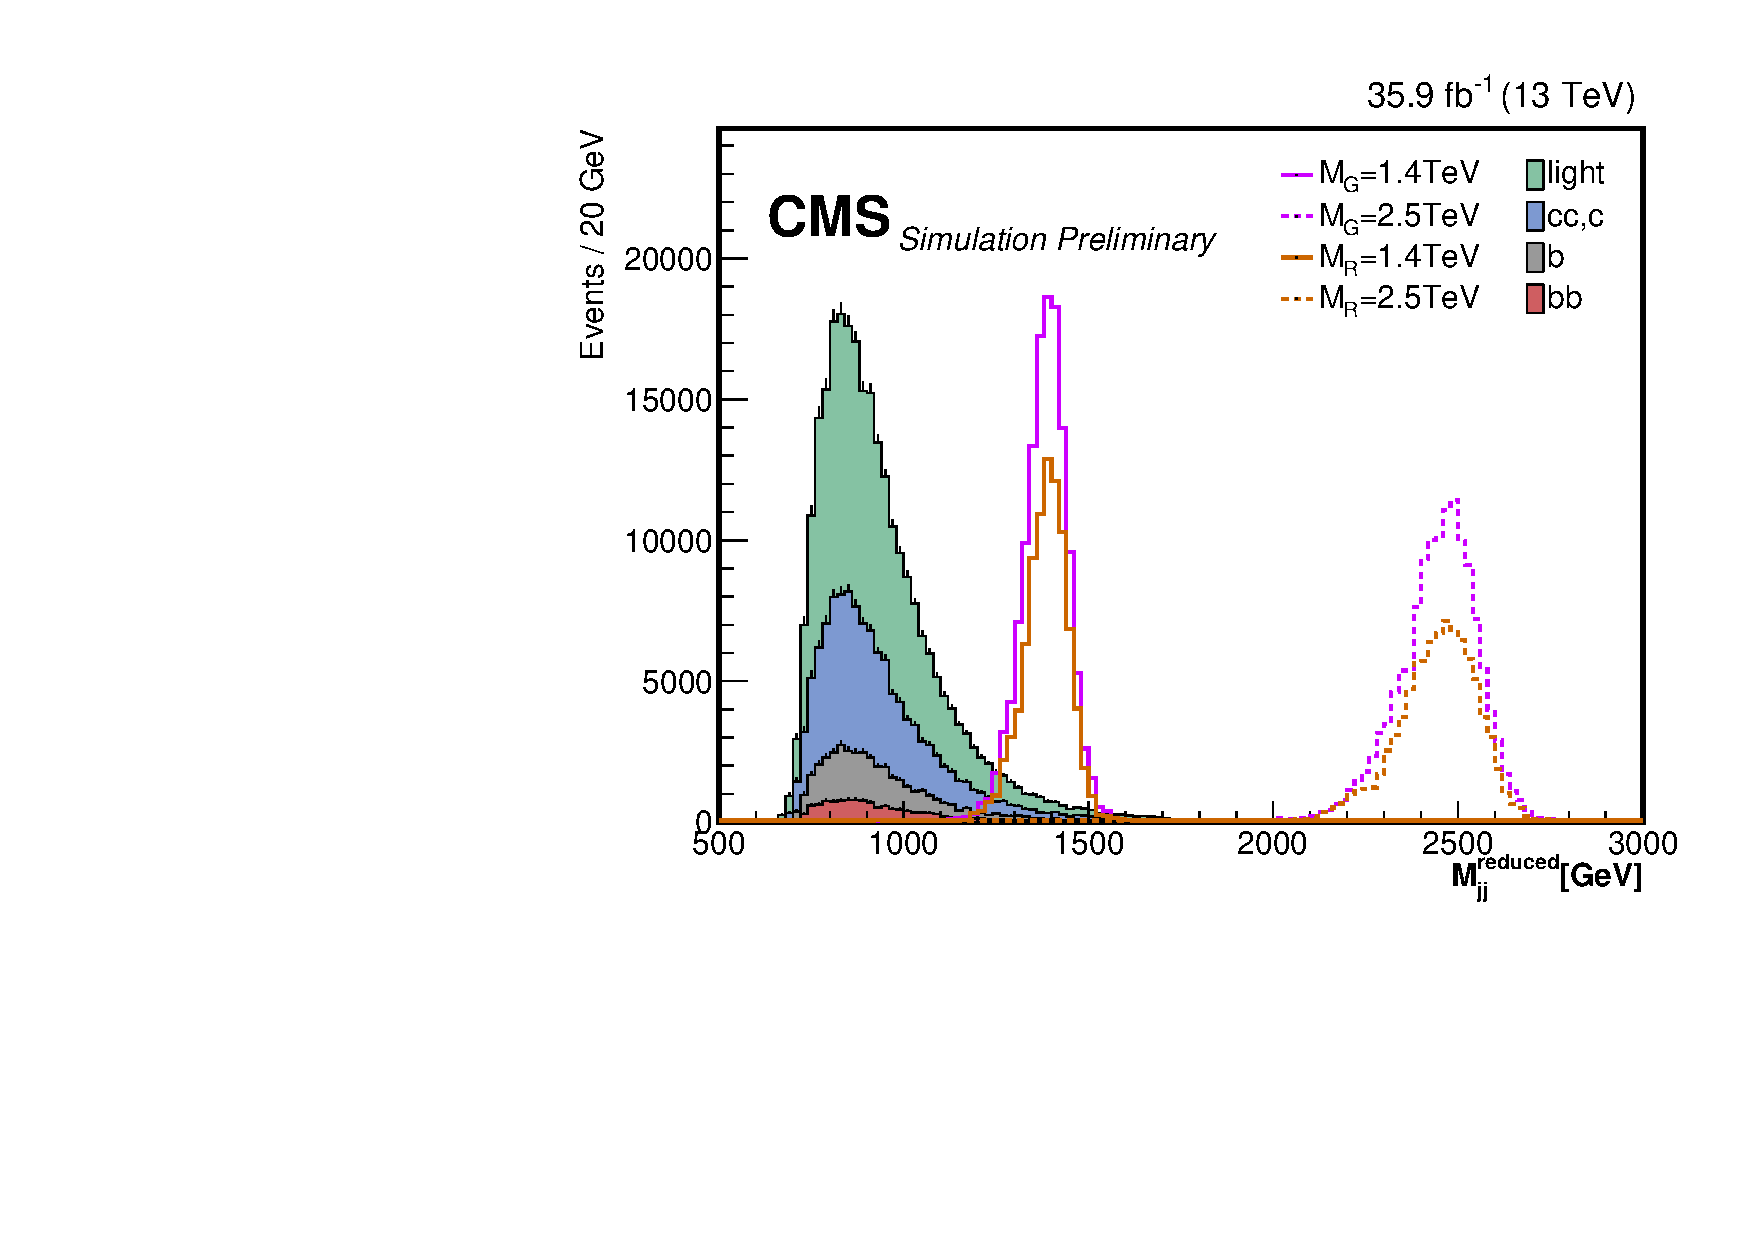
\includegraphics[width=0.5\textwidth]{Figures/MC_N1/totalMassRed.pdf} &
%    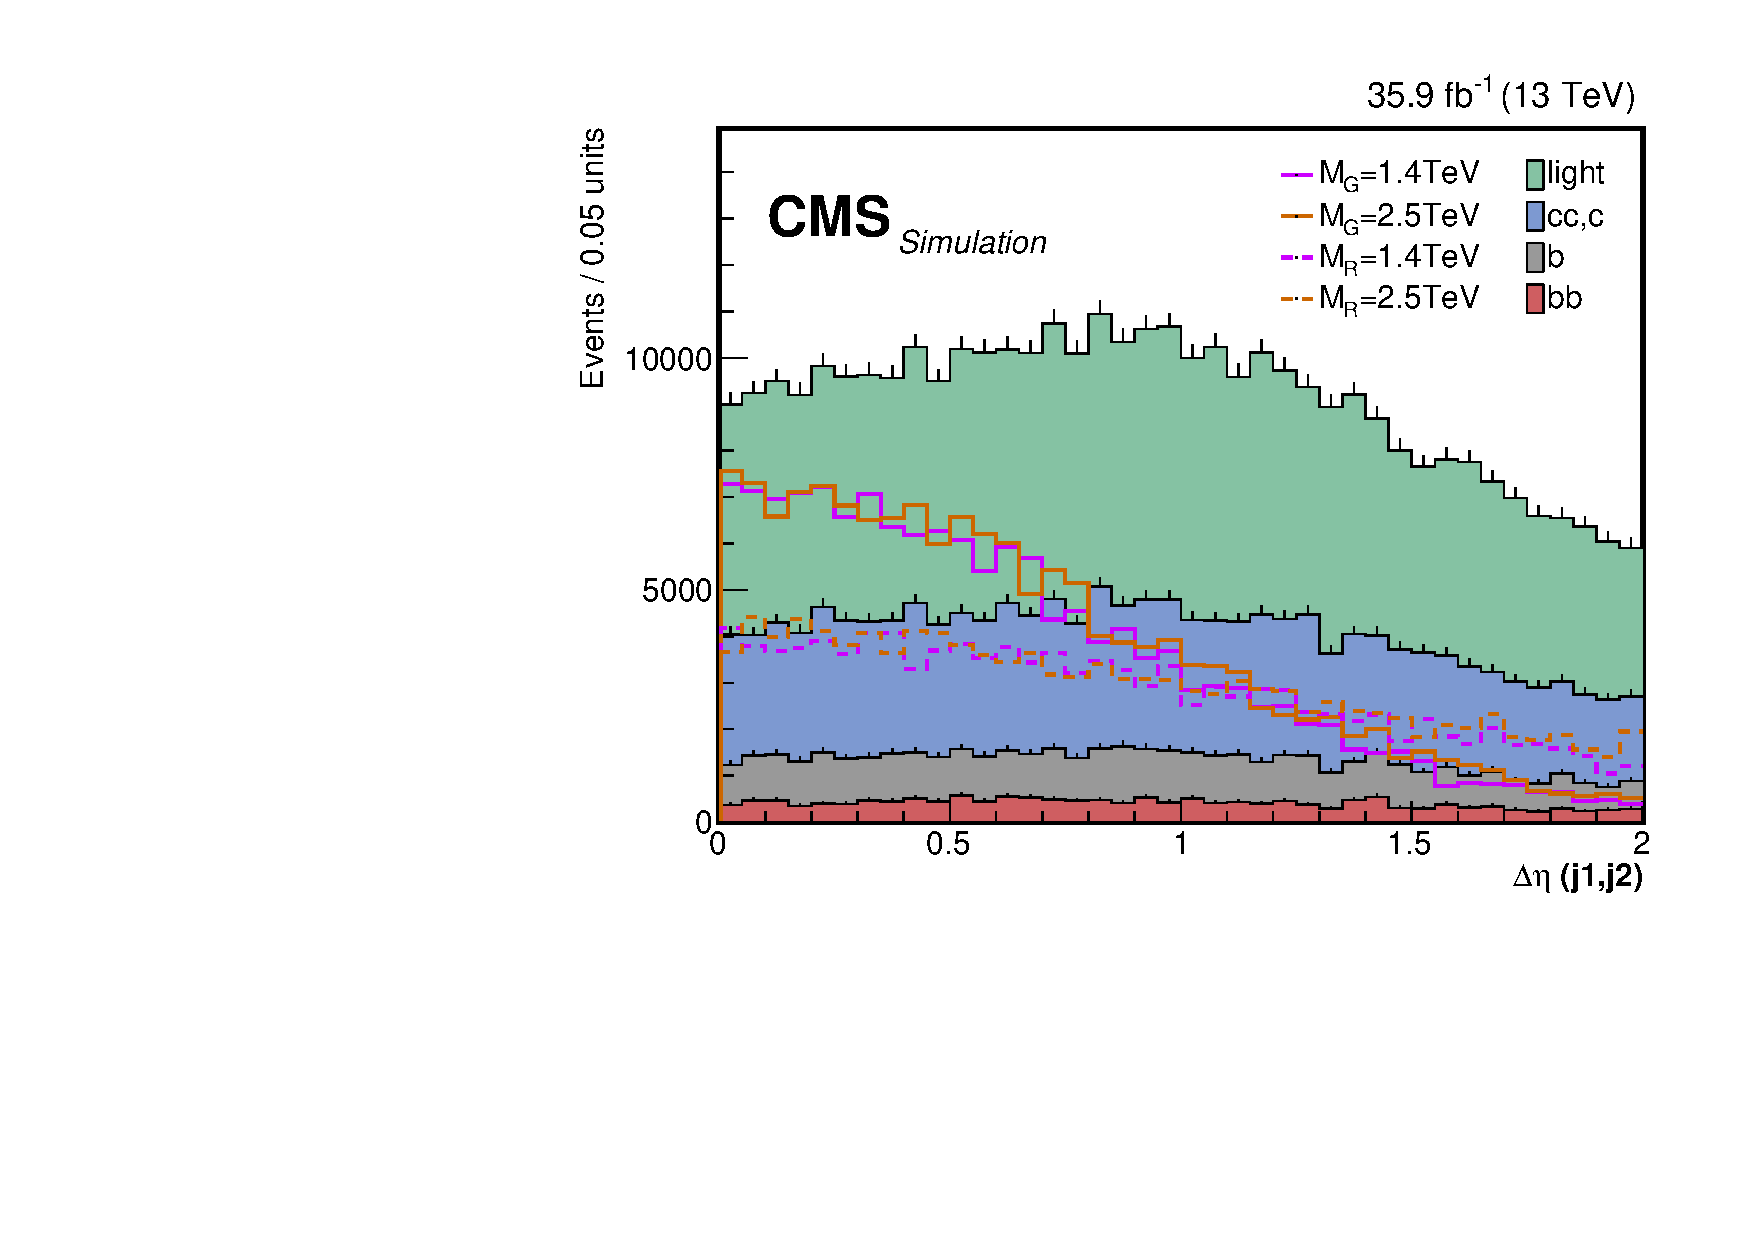
\includegraphics[width=0.5\textwidth]{Figures/MC_N1/deltaEta.pdf} \\
%  \end{tabular}
%  \caption{The comparison of signal and background. The signals of $M_{X}$ = 1.4 TeV and 2.5 TeV from both models are shown. The cross section is set to 20 pb in the figures. Multi-jet events are seperated into four categories summarized in the table 2.10. From top to buttom are the comparison of PUPPI soft-drop mass, $\tau _{21}$ of leading (left) and next leading (right) AK8 jet, the reduced mass (buttom left), and |$\Delta \eta $ (the two leading AK8 jets)| (buttom right).}
%  \label{fig:hvt_brs}
%\end{figure}